\subsection{Выборочные коэффициенты корреляции}
	\begin{table}[H]
		\centering
		\begin{tabular}{| c | c | c | c |}
			
			\hline
			$\rho=0$  & $r$      & $r_S$  & $r_Q$ \\
			\hline
			$E(z)$    & -0.01 & 0.002 & 0.0   \\
			$E(z^2)$  & 0.026 & 0.024 & 0.04  \\
			$D(z)$    & 0.051 & 0.051 & 0.051 \\
			\hline
			$\rho=0.5$ & $r$      & $r_S$  & $r_Q$ \\
			\hline
			$E(z)$    & 0.516 & 0.488 & 0.4   \\
			$E(z^2)$    & 0.267 & 0.239 & 0.16  \\
			$D(z)$      & 0.031 & 0.033 & 0.045 \\
			\hline
			$\rho=0.9$  & $r$      & $r_S$  & $r_Q$ \\
			\hline
			$E(z)$    & 0.903 & 0.88  & 0.8   \\
			$E(z^2)$    & 0.816 & 0.774 & 0.64  \\
			$D(z)$      & 0.003 & 0.005 & 0.028 \\
			\hline
			
		\end{tabular}{}
		\caption{Двумерное нормальное распределение, n = 20}
		\label{tab:n20}
	\end{table}
	
	
	\begin{table}[H]
		\centering
		\begin{tabular}{| c | c | c | c |}
			
			\hline
			$\rho = 0$ & $r$      & $r_S$  & $r_Q$ \\
			\hline
			$E(z)$    & -0.013 & -0.01 & 0.0   \\
			$E(z^2)$  & 0.008  & 0.007 & 0.004 \\
			$D(z)$    & 0.015  & 0.015 & 0.016 \\
			\hline
			$\rho = 0.5$ & $r$      & $r_S$  & $r_Q$ \\
			\hline
			$E(z)$    & 0.497 & 0.47  & 0.333 \\
			$E(z^2)$    & 0.247 & 0.221 & 0.111 \\
			$D(z)$      & 0.009 & 0.011 & 0.014 \\
			\hline
			$\rho = 0.9$ & $r$      & $r_S$  & $r_Q$ \\
			\hline
			$E(z)$    & 0.9   & 0.885 & 0.733 \\
			$E(z^2)$    & 0.81  & 0.784 & 0.538 \\
			$D(z)$      & 0.001 & 0.001 & 0.009 \\
			\hline
			
		\end{tabular}{}
		\caption{Двумерное нормальное распределение, n = 60}
		\label{tab:n60}
	\end{table}
	
	
	
	\begin{table}[H]
		\centering
		\begin{tabular}{| c | c | c | c |}
			
			\hline
			$\rho = 0$ & $r$      & $r_S$  & $r_Q$ \\
			\hline
			$E(z)$    & -0.005 & -0.004 & 0.0   \\
			$E(z^2)$  & 0.005  & 0.005  & 0.006 \\
			$D(z)$    & 0.01   & 0.01   & 0.01  \\
			\hline
			$\rho = 0.5$ & $r$      & $r_S$  & $r_Q$ \\
			\hline
			$E(z)$    & 0.496 & 0.477 & 0.32  \\
			$E(z^2)$    & 0.246 & 0.227 & 0.102 \\
			$D(z)$      & 0.006 & 0.007 & 0.009 \\
			\hline
			$\rho = 0.9$ & $r$      & $r_S$  & $r_Q$ \\
			\hline
			$E(z)$    & 0.9  & 0.887 & 0.72  \\
			$E(z^2)$    & 0.81 & 0.787 & 0.518 \\
			$D(z)$      & 0.0  & 0.001 & 0.005 \\
			\hline
			
		\end{tabular}{}
		\caption{Двумерное нормальное распределение, n = 100}
		\label{tab:n100}
	\end{table}
	
	
	\begin{table}[H]
		\centering
		\begin{tabular}{| c | c | c | c |}
			
			\hline
			$size = 20$ & $r$      & $r_{S}$ & $r_{Q}$ \\
			\hline
			$E(z)$    & 0.796 & 0.767 & 0.6   \\
			$E(z^2)$    & 0.633 & 0.588 & 0.36  \\
			$D(z)$      & 0.038 & 0.013 & 0.009 \\
			\hline
			$size = 60$ & $r$      & $r_{S}$ & $r_{Q}$ \\
			\hline
			$E(z)$    & 0.793 & 0.772 & 0.6   \\
			$E(z^2)$    & 0.629 & 0.596 & 0.36  \\
			$D(z)$      & 0.011 & 0.004 & 0.003 \\
			\hline
			$size = 100$ & $r$      & $r_{S}$ & $r_{Q}$ \\
			\hline
			$E(z)$    & 0.793 & 0.775 & 0.56  \\
			$E(z^2)$     & 0.63  & 0.6   & 0.314 \\
			$D(z)$       & 0.007 & 0.002 & 0.002 \\
			\hline
			
		\end{tabular}{}
		\caption{Смесь нормальных распределений}
		\label{tab:mix_normal}
	\end{table}
	
\subsection{Эллипсы рассеивания}
	
	\begin{figure}[H]
		\centering
		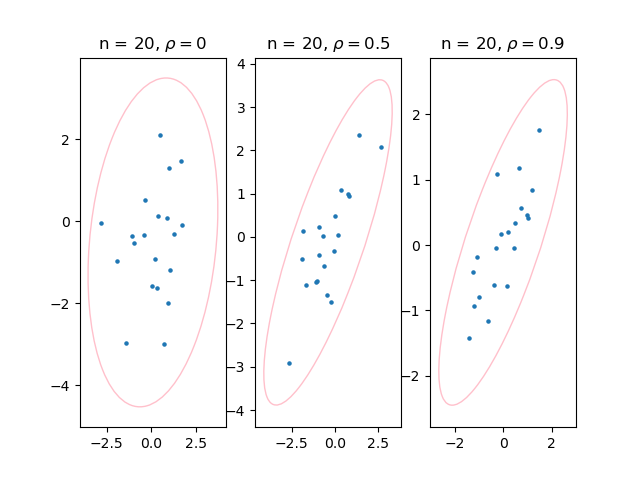
\includegraphics[width = 10cm, height = 8cm]{pics/n20.png}
		\caption{Двумерное нормальное распределение, n = 20}
		\label{fig:n20}
	\end{figure}
	
	\begin{figure}[H]
		\centering
		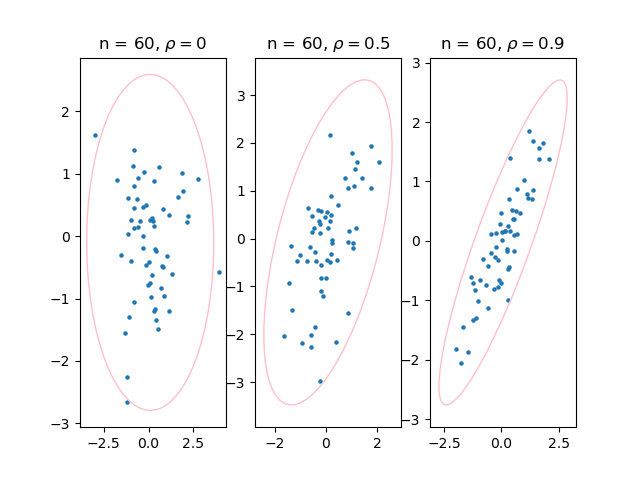
\includegraphics[width = 10cm, height = 8cm]{pics/n60.png}
		\caption{Двумерное нормальное распределение, n = 60}
		\label{fig:n60}
	\end{figure}

	\begin{figure}[H]
		\centering
		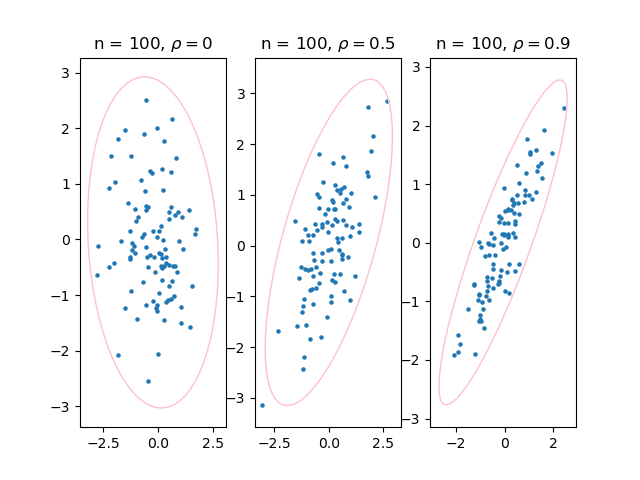
\includegraphics[width = 10cm, height = 8cm]{pics/n100.png}
		\caption{Двумерное нормальное распределение, n = 100}
		\label{fig:n100}
	\end{figure}

	
